\documentclass[12pt, letterpaper]{article}

\usepackage{hyperref}
\usepackage{graphicx}
\usepackage{float}
\usepackage{geometry}
\geometry{margin=3cm}
\usepackage[boxed]{algorithm2e}


\graphicspath{ {./images/} }
\SetKw{KwBy}{by}

\title{MPC: Find common elements in two sets of integer numbers}
\begin{document}
\maketitle

\tableofcontents
\pagebreak

\section{Introduction}
The objective of this project is to create a script to evaluate the common elements between two parties, such that neither one of them knows about the inputs of the others and where an element is a 8-bit integer.\\
\\
Given Alice's set: $AS = \{a_1, a_2, \dots, a_n\}$ and Bob's set: $BS = \{b_1, b_2, \dots, b_m\}$, our goal is for both Bob and Alice to know $RS = AS \cup BS$, without Bob knowing any of the elements $a_i \in AS$ and without Alice knowing any of the elements $b_j \in BS$.
\section{The code}
\label{sec:code}
The code for this project was built around the \href{https://github.com/ojroques/garbled-circuit}{garbled-circuit } library.
\\
Functionalities of the implemenetation:
\begin{itemize}
    \item class Alice
        \begin{itemize}
            \item \textbf{function "print"}: First Alice selects the circuit, generate the keys for the wires and a random value for each wire. Then Alice reads its input, and she exchanges with Bob the number of their inputs: N,M. At last Alice will send to Bob its input in a specific format: Given $a_1, a_2, \dots, a_n$ the inputs of Alice, she sends M times $a_1$, M times $a_2$, $\dots$, M times $a_n$.
        \end{itemize} 
    \item class Bob
        \begin{itemize}
            \item \textbf{function "send\_evaluation"}: Very similar to the print function of Alice, Bob first receives from Alice the circuit, then exchange with Alice the number of it's inputs, and finally computes the compare function. Given Bob's values: $b_1, b_2, \dots, b_m$, Bob is expected from Alice to send for N times (number of inputs of Alice), all of it's inputs; so Bob will send $b_1$ then $b_2$ then $\dots$ then $b_n$ then $b_1$, and it will repeat this N times.
        \end{itemize}
    \item class ObliviousTransfer
    \begin{itemize}
        \item \textbf{functions "get\_result", "send\_result"}: Alice and Bob perform oblivious transfer, a technique used to share with Bob only one of the two possible keys for Bob bound to a wire W.
    \end{itemize}
    \item \textbf{classes GarbledCircuit and GarbledGate}: these classes are used to generate keys and random value associated with each wire W, aswell as to compute the circuit output, given the inputs.
    \item \textbf{functions "encrypt"/"decrypt"}: Both encryption and decryption is done with the Fernet library, which provides a "Mac and Encrypt" symmetric authenticated scheme, which uses AES with CBC-MODE with a 128 bits keys, and HMAC with a 128 bits key aswell (different from the one used for AES).
    \item \textbf{class Socket\_connection\_single\_value}: create a temporary connection; used for both Alice and Bob to communicate the number of their inputs: N,M.
    \item \textbf{function "read\_input\_file"}: used to read the file containing the set of inputs of both Alice and Bob. Inputs are read as a list of integers: "1 10 251" are saved as $[1,10,251]$.
    \item \textbf{function "convert\_input\_list\_to\_nbit\_list"}: Convert inputs from a list of integers, to a list of lists, where each inner list represent an integer in binary. Ex: Given $[1,10,251]$, the result of the conversion is: $[[0,0,0,0,0,0,0,1],[0,0,0,0,1,0,1,0]],[1,1,1,1,1,0,1,1]]$
\end{itemize}
\subsection{Python version and required libraries}
\label{sec:libraries}
\begin{itemize}
    \item Python version: 3.10.9
    \item Library ZeroMQ for communications
    \item Library Fernet for encryption of garbled tables
    \item Library SymPy for prime number manipulation
\end{itemize}
\subsection{Alice communication to Bob}
\begin{algorithm}[H]
    \SetAlgoLined
     inputs\_of\_alice $\leftarrow$ read\_inputs()\;
     N $\leftarrow$ length(inputs\_of\_alice)\;
     send\_to\_Bob(N)\;
     M $\leftarrow$ receive\_from\_Bob\_number\_of\_inputs()\\
     \For{$i\gets0$ \KwTo $N$}{
        \For{$j\gets0$ \KwTo $M$}{
            \#Perform OT\\
            c $\leftarrow$ generate()\\
            send\_to\_Bob(c)\\
            $z_b$,$z_{b-1}$ $\leftarrow$ get\_from\_Bob()\\
            if($z_b$ == $z_{b-1}$): continue\\
            $r_0$,$r_1$ $\leftarrow$ generate()\\
            $c_1$ $\leftarrow$ ($g^{r_0}$, H($z_b^{r_0} \oplus k_b^0$))\\
            $c_2$ $\leftarrow$ ($g^{r_1}$, H($z_b^{r_1} \oplus k_b^1$))\\
            send\_to\_Bob(c1,c2)\\
            \#Send Alice input to Bob\\
            \# Note that Alice's inputs are not sent in clear, instead Alice sends keys: Ex $k_a^0$ stands for 0 as input\\
            send\_to\_Bob(inputs\_of\_alice[i])\\
            output $\leftarrow$ get\_result\_from\_Bob()\\
        }
        
     }
\end{algorithm}

\subsection{Bob communication to Alice}
\begin{algorithm}[H]
    \SetAlgoLined
     inputs\_of\_bob $\leftarrow$ read\_inputs()\\
    M $\leftarrow$ length(inputs\_of\_bob)\\
    send\_to\_Alice(M)\\
    N $\leftarrow$ receive\_from\_Alice\_number\_of\_inputs()\\
     \For{$i\gets0$ \KwTo $N$}{
        \For{$j\gets0$ \KwTo $M$}{
            \#Perform OT\\
            c $\leftarrow$ receive\_from\_Alice()\\
            $k$ $\leftarrow$ generate()\\
            $z_b$,$z_{b-1}$ $\leftarrow$ $g^k$, $\frac{c}{g^k}$\\
            $c_1$, $c_2$ $\leftarrow$ receive\_from\_Alice()\\
            $z_b^{r_0}$ $\leftarrow$ $(g^{r_0})^k$\\
            $z_{b-1}^{r_1}$ $\leftarrow$ $(g^{r_1})^k$\\
            $k_b^0$ $\leftarrow$ $H(z_b^{r_0}) \oplus (H(z_b^{r_0} \oplus k_b^0))$\\
            $k_b^1$ $\leftarrow$ $H(z_{b-1}^{r_1}) \oplus (H(z_{b-1}^{r_1} \oplus k_b^1))$\\
            \#Bob has access to both keys for Bob, without Alice knowing which Bob will use\\
            alice\_input $\leftarrow$ get\_alice\_input()\\
            output $\leftarrow$ compute\_output(alice\_input, inputs\_of\_bob[j], $k_b^0$, $k_b^1$)\\
            send\_output\_to\_alice(output)\\
        }
        
     }
\end{algorithm}

\section{The Compare circuit}
\label{sec:compare}
The compare circuits is a boolean circuit built using logical doors and in the code (circuits/cmp.json) is saved the compare circuit in a json form.\\
In the following sections is shown how the circuit used in the implementation described above was built and how it works, moreover it's also shown how to create a compare circuit for a general $n$-bit integer.
\subsection{The 8-bit compare circuit}
\label{section:8-bit-cmp}
Given two 8 bit values: A$=a_1,a_2,a_3,a_4,a_5,a_6,a_7,a_8$, B$=b_1,b_2,b_3,b_4,b_5,b_6,b_7,b_8$, the 8-bit compare logical circuit \ref{fig:8bit} aim is to return OUT$=1$ if A$=$B, else OUT$=0$.\\
Starting from the end of the circuit, we can see that OUT$=1$ iff every "subunit" on the left outputs 1. Each subunit is composed by 2 inputs: $a_i, b_i$, a XOR gate and a NOT gate.
\begin{figure}[h]
    \label{fig:8bit}
    \centering
    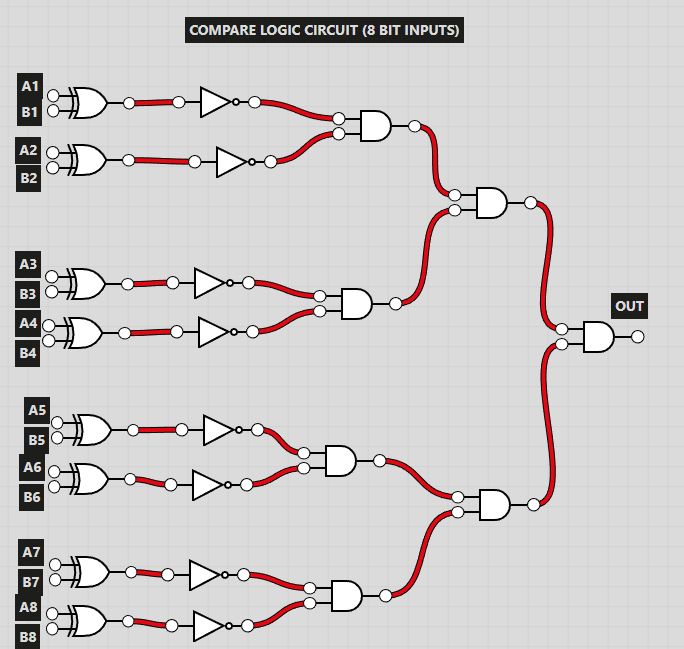
\includegraphics[width=0.6\textwidth]{8bit_circuit}
    \caption{8-bit compare logical circuit, built using \href{https://logic.ly/demo/}{logic.vy}}
\end{figure}
\\
The i-th subunit returns 1 iff $a_i=b_i=0$ or $a_i=b_i=1$ \ref{fig:XNOR}, hence OUT will be equal to 1 only if A$=$B.
\begin{figure}[H]
    \label{fig:XNOR}
    \centering
    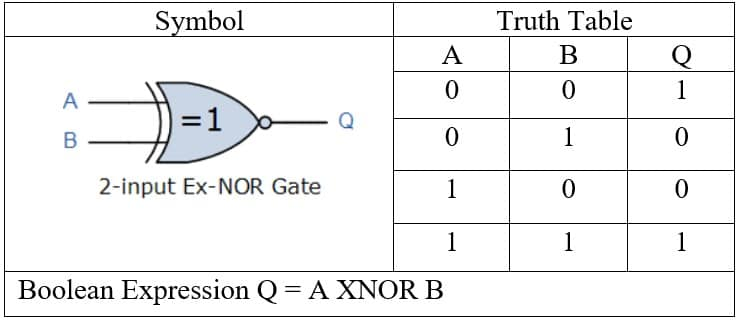
\includegraphics[width=0.6\textwidth]{XNOR}
    \caption{XNOR truth table}
\end{figure}
\subsection{How to create an n-bit compare circuit}
To build a n-bit circuit for compare it is sufficient to use "subunits" described earlier \ref{section:8-bit-cmp}.\\
Given A$=a_1,a_2,\dots,a_n$ and B$=b_1,b_2,\dots,b_n$:
\begin{enumerate}
    \item Link each i-th couple $a_i,b_i$ to a XOR and then NOT (or a XNOR) gate; we will call these "subunits", and we obtain a set $s_1,s_2,\dots,s_k$, where $s_i$ is a subunit. If a single gate remains out add it into the set of couples of subunits as a single subunit;
    \item Subdivide the subunits into couples $(s_1,s_2),(s_3,s_4),\dots,(s_{k-1},s_k)$, and link each couple to an AND gate.
    \item Keep going subdividing into couples and linking them to AND doors until you have no more couples. 
\end{enumerate}
In the end you will end up with a logic circuit for compare for n-bits.

\section{Running the code}
\label{sec:run}
\subsection{Insert inputs}
You can insert inputs in the files inside the folder "inputs/", that are named after both Alice and Bob, which contains respectively the set of integers of Alice and the set of integers of Bob which have to be compared.\\
\\
Inputs are integer numbers $\in [0,255]$ interspaced by a blank space.\\
Example: "65 1 0 155 32 255 1 3 1 0 83" (without "")
\subsection{Run the script}
\begin{enumerate}
    \item be sure that ports 4080, 40800 and 40801 aren't currently occupied;
    \item open the terminal for Bob and enter an enviroment with the required libraries \ref{sec:libraries};
    \item execute Bob: "python main.py bob" or "./main.py bob", now Bob will keep listening for requests from Alice;
    \item open the terminal for Alice and enter an enviroment with the required libraries \ref{sec:libraries};
    \item execute Alice: "python main.py alice -c circuits/cmp.json" or  "./main.py alice -c circuits/cmp.json";
    \item if you want to run the program with different inputs, it's sufficient you insert the inputs and re-run Alice, you don't need to restart Bob.
\end{enumerate}
At the end of the computation both Bob and Alice will print the common set of elements.

\section{Conclusions}
This project accomplished it's target objective: creating a working MPC enviroment for the "compare" function between sets of 8-bit integer numbers (chapter \ref{sec:code}).\\
In chapter \ref{sec:compare} it is shown how to create a general version of the compare circuit that could extend the current integer range $[0,255]$, to the range $[0,2^i]$ for a i-bits compare circuit, and finally in chapter \ref{sec:run} we showed how to run the code and insert inputs.
\\
\\
A possible future development is to make this code also work for 8 bits floating point numbers. In order to do so the compare circuit would remain the same, but we would need to reconognize if the input that was received was an integer or a float (we could write a lexer/parser couple), and then to process them accordingly.

\end{document}

